\subsection{Unknown Input Observer (UIO)} \label{sec:UIO}
Disturbances and modeling errors may cause discrepancies between the actual system and the descriptor mathematical model. Linearization and simplifications which make the system more manageable may lead to such uncertainties. Uncertainties can have an effect on the system dynamic behavior. During observer design, these uncertainties can be considered as unknown inputs. The observer can be designed to make the system state estimate error converge to zero in the presence of such unknown inputs. The linearized system dynamics is described according to equations \ref{stateObs} and \ref{eq:ui2}.
  
%A residual, fault indicator, based on observer design can be robust regarding the unknown input signals by making the effect of unknown inputs (UI) insensitive to the residual and thus making possible to maximize the detectability of a fault. The dynamic equation of the system can be written as  

%\nomenclature[A]{\textbf{UI}}{Unknown Input}
%

\nomenclature[AU]{\textbf{UIO}}{Unknown Input Observer }

\begin{equation}
\dot{\vec{x}} = \underline A\vec{x}+\underline B \vec{u}+\underline E\vec{d}
\label{stateObs}
\end{equation}
\begin{equation}
\vec{y} = \underline C \vec{x}
\label{eq:ui2}
\end{equation}
%
where $\underline A$ ,$\underline B$ and $ \underline C $ are the system matrix, input and output matrix respectively and $\underline E$ is the distribution matrix of the unknown input (disturbance) $\vec{d}$. Furthermore, $\vec{x}$ is the state vector, $\vec{u}$ is the input vector and $\vec{y}$ is the output vector. The time dependency of the variables has been suppressed in order to relax the notation. Following \cite{UIO}, 
%
%
\\
\textit{An observer is defined as Unknown Input Observer for a system described by \eqref{stateObs} if the state estimation error vector $e$ approaches zero asymptotically regardless of the presence of the unknown input }
\\
The full order observer dynamics is set up according to equations \ref{stateObs1} and \ref{stateObs2}.
\begin{equation}
\dot{\vec{z}} = \underline F\vec{z}+\underline{TB} \vec{u}+\underline K\vec{y}
\label{stateObs1}
\end{equation}
\begin{equation}
\hat{\vec{x}} = \vec{z} + \underline H \vec{x}
\label{stateObs2}
\end{equation}

with $\hat{\vec{x}}$ being the state estimate and $\vec{z}$ the state of the observer. When \eqref{stateObs1} is an observer for the system given by \eqref{stateObs} the dynamics of the error  vector ($\vec{e} = \vec{x} - \hat{\vec{x}}$) can be written according to equation \ref{errordynamics} \cite{UIO}.
\begin{equation}
\dot{\vec{e}}= (\underline A-\underline H \underline C \underline A-\underline K1 \underline C)\vec{e} + (\underline A-\underline H \underline C \underline A-\underline K1 \underline C - \underline F)\vec{z}+ ((\underline A-\underline H \underline C \underline A-\underline K1 \underline C )\underline H-\underline K2)\vec{y}
\label{errordynamics}
\end{equation}
\begin{equation*}
+ (\underline I - \underline {HC} - \underline T)\underline B\vec{u}	+(\underline I -\underline H\underline C)\underline E \vec{d}
\label{errordynamics45}
\end{equation*}
in the above equation the utility of $\vec{x}  = \vec{e} + \hat{\vec{x}} = \vec{e} + \underline H\vec{y}+\vec{z}$ is used. The estimation error may converge to zero if the following conditions hold true:
%
\begin{equation}
\underline F = \underline A-\underline H \underline C \underline A-\underline K1 \underline C
\label{errordynamics3}
\end{equation}
\begin{equation}
(\underline I - \underline{HC})\underline E = 0
\label{errordynamics4}
\end{equation}
\begin{equation}
\underline T = (\underline I - \underline H\underline C)
\label{errordynamics5}
\end{equation}
\begin{equation}
\underline K = \underline K_{1} +\underline K_{2}
\label{errordynamics6}
\end{equation}
\begin{equation}
\underline K_{2} =\underline F \underline H 
\label{errordynamics7}
\end{equation}
where $\underline K_{1}$ is designed freely by pole placement to give desired eigenvalues of the observer. The error dynamics if equations \ref{errordynamics4}-\ref{errordynamics7} hold true can now be written as 
\begin{equation}
\dot{\vec{e}} = \underline F \vec{e}
\label{errordynamics8}
\end{equation}
consequently if the eigenvalues of $\underline F$ are to the left half plane, the error converges exponentially to zero. 

A solution to \eqref{errordynamics4} is given by making use of the Moore-Penrose pseudo-inverse as
\begin{equation}
\underline H = \underline E (\underline{CE})^\dagger
\label{errordynamics9}
\end{equation}
with $(\underline{CE})^{+} = [(\underline{CE})^{T} (\underline{CE})]^{-1}\underline{CE})^{T} $.
A sufficient and necessary condition for the UIO existence is that the number of independent unknown inputs can not be larger than the number of independent measurements which leads to
\begin{equation}
rank (\underline{CE}) =rank( \underline E) 
\label{errordynamics10}
\end{equation}
and by denoting $\underline A_1 = \underline A - \underline{HCA} $ that the pair $(\underline {CA}_1)$ is detectable and thus $F$ can have stable roots.


\subsubsection{Residual Generation}

In order to be able to detect faults, a residual signal is set up.  The residual should converge to zero in the presence of $\vec{d}$ unknown input and the absence of faults. In order to make the faults strong detectable, the residual should not converge to zero in the presence of faults. The residual is defined as
%The residual is used for fault detection and isolation thus should be decoupled from the unknown inputs(disturbances). The residual can be written as
\begin{equation*}
\vec{r} = \vec{y} - \underline C \hat{\vec{x}} 
\label{errordynamics11} = 
= \vec{y} - \underline C (\vec{z} + \underline{H} \vec{y} ) 
= (\underline I  -\underline{ CH})\vec{y}   -\underline C \vec{z} 
\end{equation*}

which does not depend on the disturbance vector. Residual thresholding can be applied to detect faults.
% A simple threshold can be applied such that for the faulty case, if the magnitude of the residual is larger than the threshold then a fault has been occurred as
%$\{\lVert \vec{r}\rVert \geq threshold \}$ else if $\{\lVert \vec{r}\rVert < threshold \}$ then the system is fault free.
Figure 7.8. illustrates the nominal unknown input observer with a block diagram. 
%of the nominal system and the observer can be seen along with the residual generator
\begin{figure}[H]
	\centering
	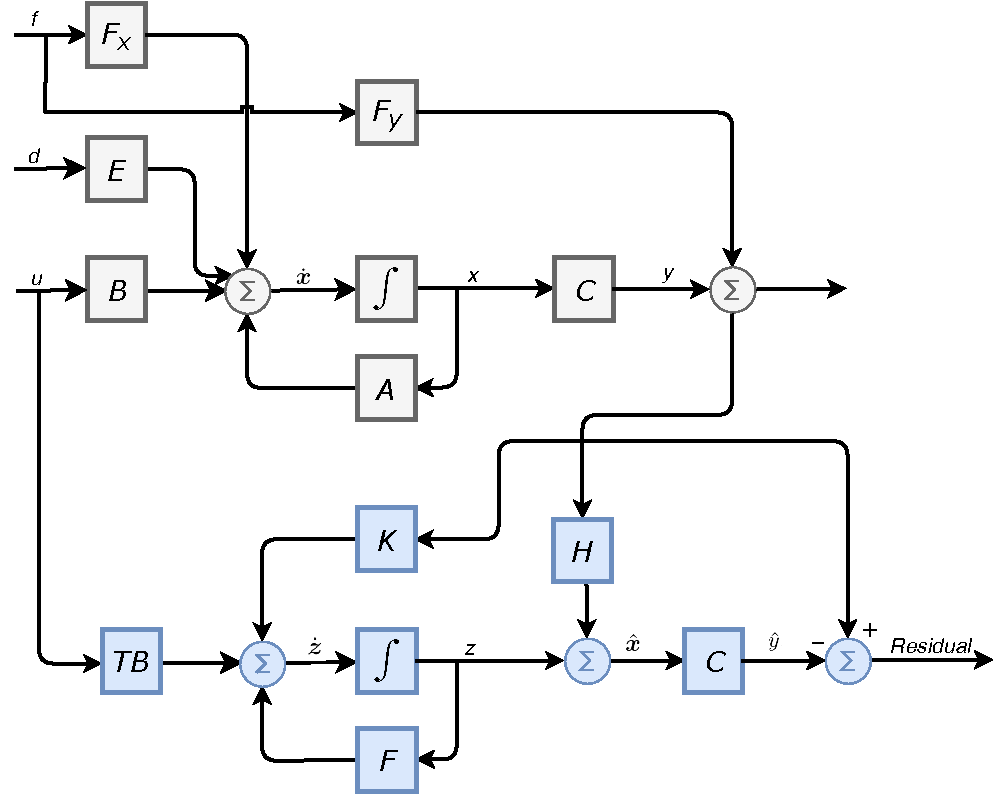
\includegraphics[width=0.8\linewidth]{figures/UIO_new}
	\caption{Observer based residual generator}
	\label{fig:residualobs}
\end{figure}

%Moreover, in figure \ref{fig:residualobstest} it can be seen how the state error converge asymptotically to zero from the initial conditions along with a change in the attitude of the satellite after 70 seconds.

%\begin{figure}[H]
%	\centering
%	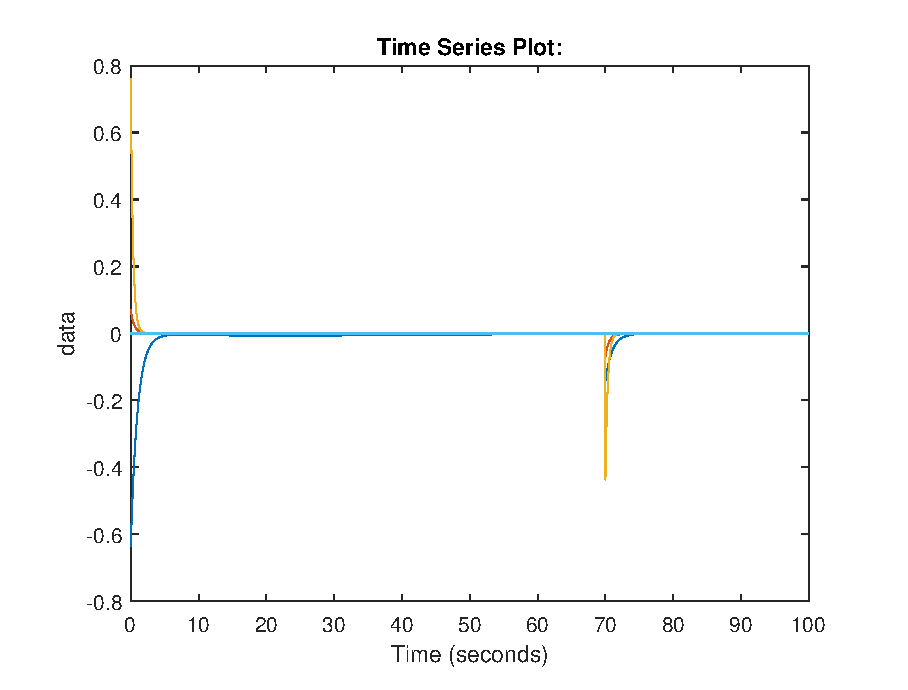
\includegraphics[width=0.7\linewidth]{figures/obstest}
%	\caption{Convergence of the state estimation error to zero with the disturbance been decoupled}
%	\label{fig:residualobstest}
%\end{figure}

Actuator fault isolation is possible assuming that all the sensors are fault free. Sensor fault isolation is possible assuming that the actuators are fault free. A descriptor model of the overall system with actuator fault can be written as given in equation \ref{stateObs}.
\begin{equation}
\dot{\vec{x}} = \underline A\vec{x}+\underline B \vec{u}+\underline E\vec{d} + \underline B\vec{f_{act}}
\label{stateObs34}
\end{equation}
where $\vec{f_{act}}$ represents the actuator faults. 

%In order to isolate faults, separate UIOs need to be constructed for each actuator. The observer matrices are adjusted for each actuator by deleting the column of the matrix B corresponding to the actuator, namely $\vec{b_{i}}$ and incorporating this along with the disturbance distribution matrix as
%\begin{equation*}
%E^{i} = [ E  \vec{b_{i}}]
%\label{errordynamics14}
%\end{equation*}
%and furthermore, the $i_{th}$ component of the input vector $u_{i}$ is incorporated to the disturbance vector as 
%\begin{flalign*}
%\begin{bmatrix}
%\vec{d} \\ u_{i}+f^{i}_{act}
%\end{bmatrix}
%\end{flalign*} 
%leading to a bank of observers with each residual actuated by 2 inputs(without $i_{th}$) and all outputs. The detection of the fault is made by applying a threshold as  $\{\lVert r^{i}\rVert < Thr^{i} \}$ else if $\{\lVert r^{k}\rVert \geq Thr^{k} \}$ with $k = 1,...i-1,..i+1,5..r$.
%
%\todo{is the last paragraph ok?}

%\subsection{CUSUM algorithm and change detection} 
%The evaluation of the residual which determines if the %actuator is faulty or fault free is based on the %cumulative sum (CUSUM), a sequential hypothesis %testing technique to detect changes on the noisy %signal. By changes are accounted changes on the mean %of the original signal. 



% \begin{figure}[H]
%	\centering
% 	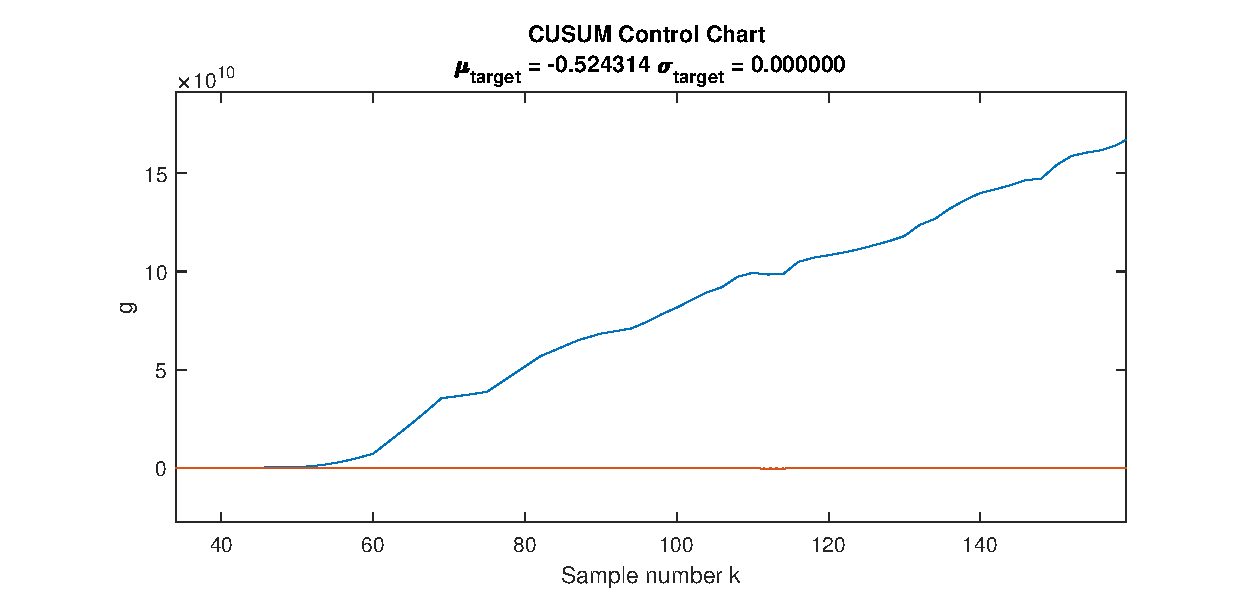
\includegraphics[width=0.7\linewidth]{figures/cusum1}
% 	\caption{CUSUM output with fault on the z axis magnetorquer at 40s }
%	\label{fig:cusum1}
%\end{figure}  



\subsection{Application of Unknown Input Observer}
\label{sec:UIO_App}


%\todo{discuss articles a bit}
%\todo{should we show the equations in more detail?}
%\todo{short model derivation}


The present chapter discusses how to apply unknown input observer (UIO) theory to the satellite functioning in nadir pointing control goal. The regular UIO uses linear model, however the satellite system is highly nonlinear.  During one orbit, the orientation of the nadir pointing satellite rotates by $360^o$. By choosing the appropriate reference frame, this rotation can be eliminated from attitude dynamics. In local vertical, local horizontal frame (LVLH), the nadir pointing satellite keeps its attitude. This opens an opportunity to use linear approximation of the trigonometric nonlinearities in the satellite dynamic equations. The operating point should be chosen as nadir pointing, and if the attitude stays near enough to the operating point, the model stays quite accurate.


Yang's article on desaturation \cite{DesatYang} describes a model that can be effective for UIO. The $\underline{A}$ matrix of the model is constant, so the UIO matrices can be derived as described in \ref{sec:UIO}. The model detaches the orbit angular velocity from the dynamics according to equation \ref{eq:angDetach}.

\begin{equation}
\label{eq:angDetach}
\vec{\omega} = \vec{_I^{lv}\omega} + \vec{_{lv}^s\omega}
\end{equation}

where $\vec{_I^{lv}\omega}$ is the angular velocity of the LVLH frame compared to the inertial frame and $\vec{_{lv}^s\omega}$ is the angular velocity of the body frame compared to the LVLH frame. $\underline{B}(t)$ includes Earth's local magnetic field, so it has to be updated at every sample. The model has been altered to include the unknown inputs and faults, furthermore the gravity gradient torque is handled outside of the system matrix $\underline{A}$.

\begin{equation}
\vec{\dot{x}} =
\underline{A}\vec{x} + \underline{B}(t)\vec{u} + \underline{E} \vec{d} + \underline{F}_x \vec{f_y} 
\label{eq:uioagain}
\end{equation}

\begin{equation}
\vec{y} =
\underline{C}\vec{x} + \underline{F}_y \vec{f_y} 
\label{eq:uioagain2}
\end{equation}

 For the detailed matrices of the model used for designing the observer, please refer to appendix \ref{sec:UIO_deriv}.

%
%\tiny
%\begin{align}
%\begin{bmatrix}
%\vec{_{lv}^s\dot{\omega}} \\
%\vec{\dot{\omega}_{rw} } \\
%\vec{\dot{q}_{1:3}}
%\end{bmatrix} 
% \nonumber\\
%= \begin{bmatrix}
%0 & 0 & \omega_o\frac{I_1 - I_2 + I_3}{-I_1} & 0.58\omega_o\frac{I_w}{I_1} & 0.58\omega_o\frac{I_w}{I_1} & 0.58\omega_o\frac{I_w}{I_1} & -\omega_o\frac{I_w}{I_1} & 2\omega_o^2\frac{I_3 - I_2}{I_1} & 0 & 0 \\
%0 & 0 &	0 & 0 & 0 &	0 & 0 &  0 &  0 & 0\\
% \omega_o\frac{I_1 - I_2 + I_3}{I_3}  & 0 & 0 &  0.81\omega_o\frac{I_w}{I_3} & 0.77\omega_o\frac{I_w}{I_3} & 0.77\omega_o\frac{I_w}{I_3} &	0 & 0 & 0 & 2\omega_o^2\frac{I_1 - I_2}{I_3}\\
%0 & 0 &	0  & 0 & 0 & 0 & 0 & 0 & 0& 0\\
%0 & 0 &	0  & 0 & 0 & 0 & 0 & 0 & 0& 0 \\
%0 & 0 &	0 & 0 & 0 & 0 & 0 & 0 & 0& 0\\
%0 & 0 &	0 & 0 & 0 & 0 & 0 & 0 & 0& 0\\
%0.5 & 0 &	0 & 0 & 0 & 0 & 0 & 0 & 0& 0 \\
%0 & 0.5 &	0& 0 & 0 & 0 & 0 & 0 & 0& 0 \\
%0 & 0 &	0.5 & 0 & 0 & 0 & 0 & 0 & 0& 0\\
%\end{bmatrix}
%\begin{bmatrix}
%_{lv}^s\omega_1 \\
%_{lv}^s\omega_2 \\
%_{lv}^s\omega_3 \\
%\omega_{rw,1} \\
%\omega_{rw,2} \\
%\omega_{rw,3} \\
%\omega_{rw,4} \\
%q_1 \\
%q_2 \\
%q_3 
%\end{bmatrix}
% \\
% \nonumber
%+
%\begin{bmatrix}
%0.81I_1^{-1} & 0.77I_1^{-1} & 0.77I_1^{-1} & 0 & 0 & \frac{b_3}{I_1} & -\frac{b_2}{I_1}	& I_1^{-1} & 0 & 0\\
%0 & 0.125I_2^{-1} & -0.125I_2^{-1} & 0 & - \frac{b_3}{I_2} & 0 &  \frac{b_1}{I_2} & 0 & I_2^{-1} & 0\\ 
%-0.58I_3^{-1} & -0.58 I_3^{-1} & -0.58 I_3^{-1} & I_3^{-1} &  \frac{b_2}{I_3} &  -\frac{b_1}{I_3} & 0 & 0 & 0 & I_3^{-1} \\  
%I_w^{-1} & 0 & 0& 0 & 0 & 0 & 0 & 0 & 0 & 0 \\
%0 & I_w^{-1} & 0& 0 & 0 & 0 & 0 & 0 & 0 & 0 \\ 
%0 & 0 & I_w^{-1} & 0 & 0 & 0 & 0 & 0 & 0 & 0\\  
%0 & 0 & 0 &  I_w^{-1} & 0& 0 & 0 & 0 & 0 & 0\\
%0 & 0 & 0 & 0 & 0& 0 & 0 & 0 & 0 & 0\\
%0 & 0 & 0 & 0 & 0& 0 & 0 & 0 & 0 & 0\\
%0 & 0 & 0 & 0 & 0& 0 & 0 & 0 & 0 & 0
%\end{bmatrix}
%\begin{bmatrix}
%N_{rw,1} \\
%N_{rw,2} \\
%N_{rw,3}\\
%N_{rw,4}\\
%\m_{mt,1} \\
%\m_{mt,2} \\
%\m_{mt,3} \\
%N^{est}_{dist,1} \\
%N^{est}_{dist,2} \\
%N^{est}_{dist,3}
%\end{bmatrix}
%+
%\\
%\nonumber
%\begin{bmatrix}
%I_1^{-1} & 0 & 0 \\
%0 & I_2^{-1} & 0 \\
%0 & 0 & I_3^{-1}\\
%0 & 0 & 0 \\
%0 & 0 & 0 \\
%0 & 0 & 0 \\
%0 & 0 & 0 \\
%0 & 0 & 0 \\
%0 & 0 & 0 
%\end{bmatrix}
%\begin{bmatrix}
%N^{est \ error}_{dist,1} \\
%N^{est \ error}_{dist,2} \\
%N^{est \ error}_{dist,3}\\
%\end{bmatrix}
% \\
% + 
% \begin{bmatrix}
%0.81I_1^{-1} & 0.77I_1^{-1} & 0.77I_1^{-1} & 0 & 0 & \frac{b_3}{I_1} & -\frac{b_2}{I_1}\\
%0 & 0.125I_2^{-1} & -0.125I_2^{-1} & 0 & - \frac{b_3}{I_2} & 0 &  \frac{b_1}{I_2} \\ 
% -0.58I_3^{-1} & -0.58 I_3^{-1} & -0.58 I_3^{-1} & I_3^{-1} &  \frac{b_2}{I_3} &  -\frac{b_1}{I_3} & 0 \\  
% I_w^{-1} & 0 & 0 & 0 & 0 & 0 \\
% 0 & I_w^{-1} & 0 & 0 & 0 & 0 \\ 
% 0 & 0 & I_w^{-1} & 0& 0 & 0 & 0 \\  
% 0 & 0 & 0 & I_w^{-1} & 0 & 0 & 0 \\
% 0 & 0 & 0 & 0 & 0 & 0& 0 \\
% 0 & 0 & 0 & 0 & 0& 0 & 0 \\
% \end{bmatrix}
% \begin{bmatrix}
% N^{fault}_{rw,1} \\
% N^{fault}_{rw,2} \\
% N^{fault}_{rw,3}\\
% N^{fault}_{rw,4}\\
% \m^{fault}_{mt,1} \\
% \m^{fault}_{mt,2} \\
% \m^{fault}_{mt,3} 
% \end{bmatrix}
%\label{eq:uioMatrices}
%\end{align}
%\normalsize

where $I_w$ is the reaction wheel axial moment of inertia, $\omega_o$ is the angular velocity of the orbit, $I_i$ is the satellite moment of inertia along $i$th principal axis. $\underline{C}$ is an identity matrix. 

If the UIO design algorithm is followed, without fault the residual converges to zero, as shown in figure 7.9 a. If the angular velocity estimate is wrong, i.e. $\underline{F}_y \vec{f_y}$ is nonzero, the residual doesn't converge to zero. Figure 7.10 a. shows the residual for an error in angular velocity estimate. The angular velocity of the satellite is estimated through and sensor fusion and filtering, the details of which is out of the scope of the present thesis.

The UIO dynamics are designed to make the residual converge to zero in the presence of unknown input $\vec{d}$. The fact that the disturbances and magnetorquer faults affect the same state variables $\vec{_{lv}^s\dot{\omega}}$ means that the system cannot distinguish the magnetorquer fault from the disturbances, thus they cannot be decoupled.

An experiment was made to investigate if ignoring the unknown torque disturbances, is it possible to distinguish magnetorquer faults through thresholding. The $\underline{E}$ was modified to a zero matrix, then the observer was redesigned accordingly. This essentially makes the observer stop being an UIO. In the test, $N^{est \ error}_{dist}$ was simulated as a constant vector with a magnitude of $1 nNm$, around $2\%$ of $\vec{N_{dist} }$, while the magnetorquer magnetic moment fault $\m^{fault}_{mt,1}$ error was a constant $10 mJ/T$, a magnitude that would occur at rather high reaction wheel speed due to desaturation torque demand. Figure  7.10 a. shows the residual when only the disturbance is present, figure 7.10.b. shows the residual when a fault occurs at 800 second intervals following a square signal. The residual for the fault is orders of magnitude higher than for the disturbance, however the residual from the disturbance keeps growing and growing through many orbits. This means that thresholding is not effective for magnetorquer fault detection in the long term with this observer.

%\todo{what about RW fault?}

\nomenclature[SIw]{$I_w$}{Reaction wheel axial moment of inertia}

\nomenclature[Somegao]{$\omega_o$}{Orbit angular velocity}

\begin{figure}[H]
	\begin{subfigure}{0.5\linewidth}
			\centering
		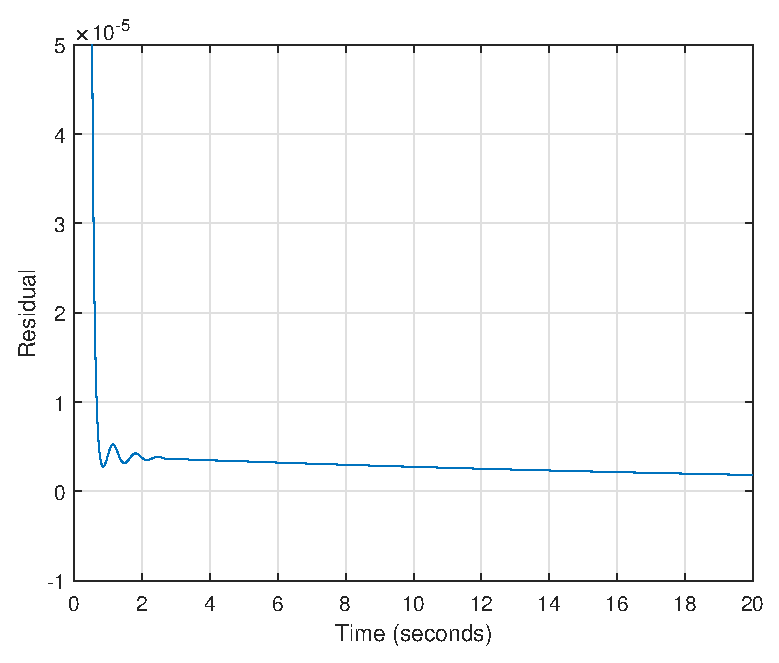
\includegraphics[width=1\linewidth]{figures/nosensfault_res}
		\label{fig:nosensfault_res}		
		\caption{}
	\end{subfigure}
		\begin{subfigure}{0.5\linewidth}
	\centering
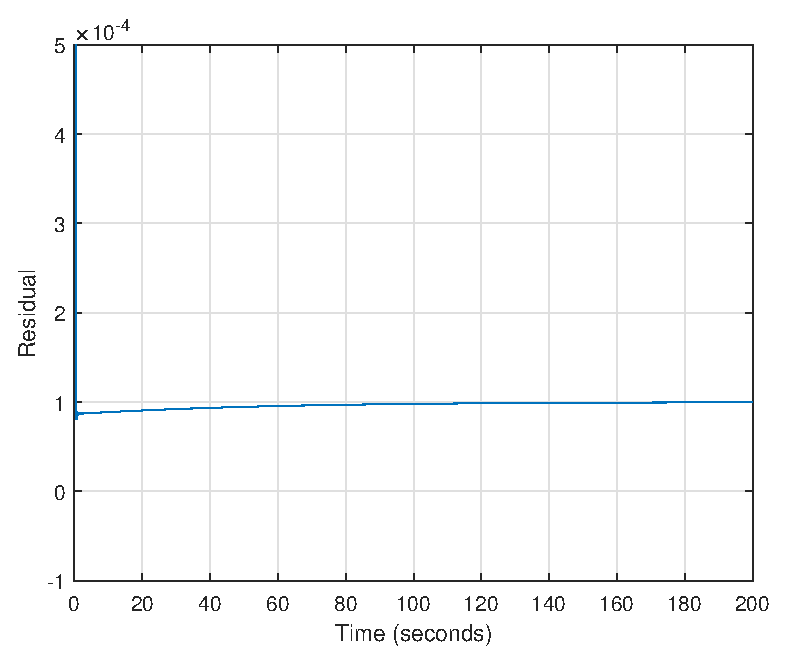
\includegraphics[width=1\linewidth]{figures/sensfault_res}
\label{fig:sensfault_res}	
\caption{}
	\end{subfigure}
\caption{7.9 a. presents how the residual converges to zero when disturbance is present and fault is absent. 7.9 b. presents the residual in case of a fault in angular velocity estimation.}
\end{figure}

%\begin{figure}[H]
%	\centering
%	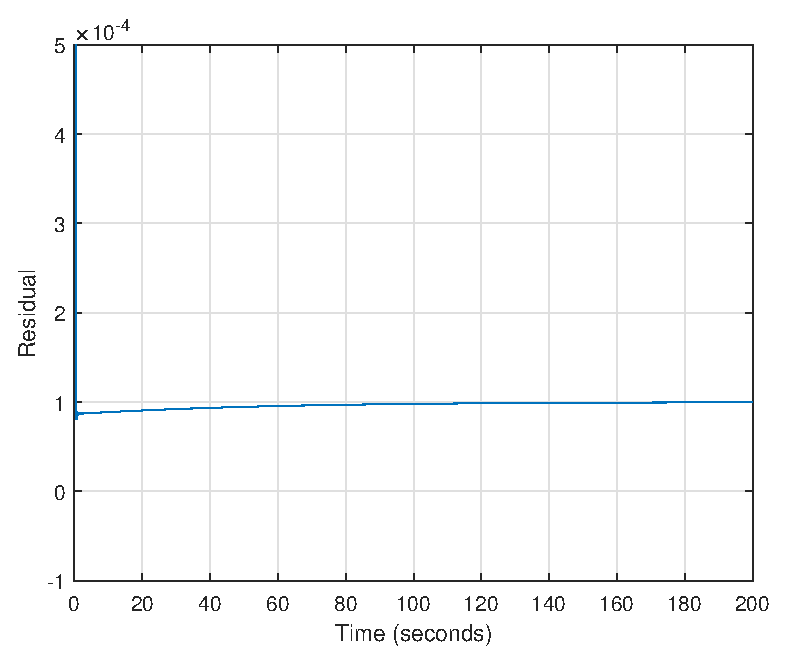
\includegraphics[width=0.7\linewidth]{figures/sensfault_res}
%	\caption{sensor fault 0.1 ang vel x excess}
%	\label{fig:}
%\end{figure}

\begin{figure}[H]
	\begin{subfigure}{0.5\linewidth}
	\centering
	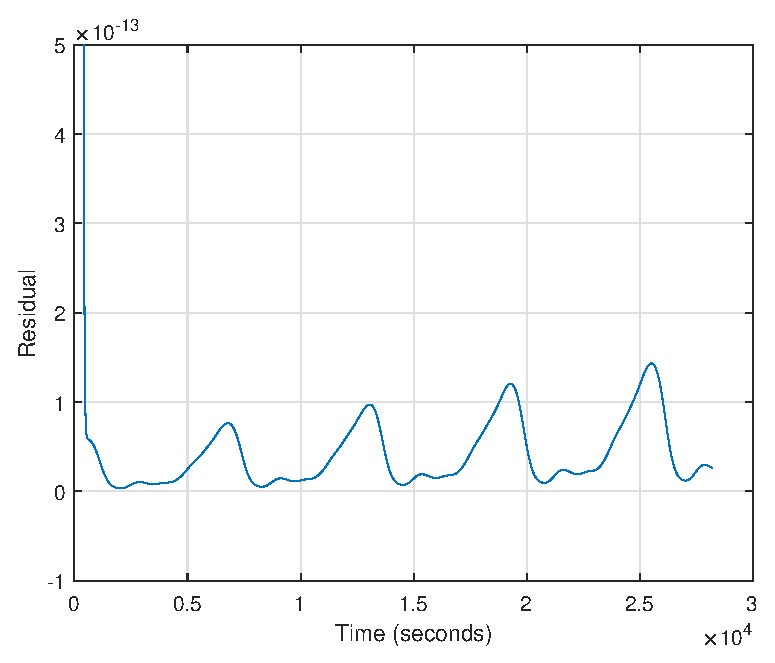
\includegraphics[width=1\linewidth]{figures/constdistonly_res}
	\label{fig:residualdist}	
	\caption{}
	\end{subfigure}
	\begin{subfigure}{0.5\linewidth}
	\centering
	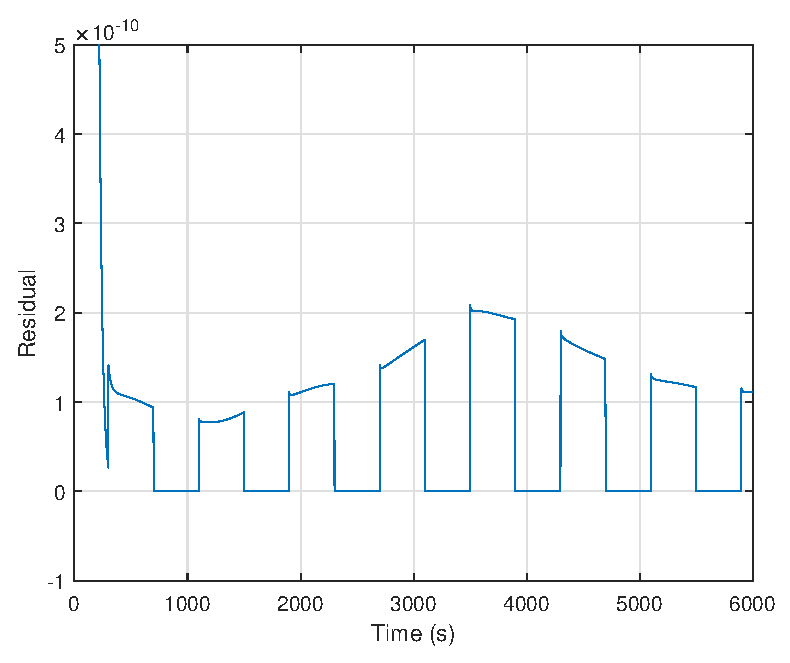
\includegraphics[width=1\linewidth]{figures/mt_fault_res}
	\label{fig:residualmt}
	\caption{}
	\end{subfigure}
\caption{7.10.a. presents the residual of the observer without torque disturbance convergence when only disturbance torque estimate is present. 7.10.b. presents the residual with periodically occurring magnetorquer fault. The order of magnitude of the residual in 7.10.a. is 3 times as big.}
\end{figure}

%\begin{figure}[H]
%	\centering
%	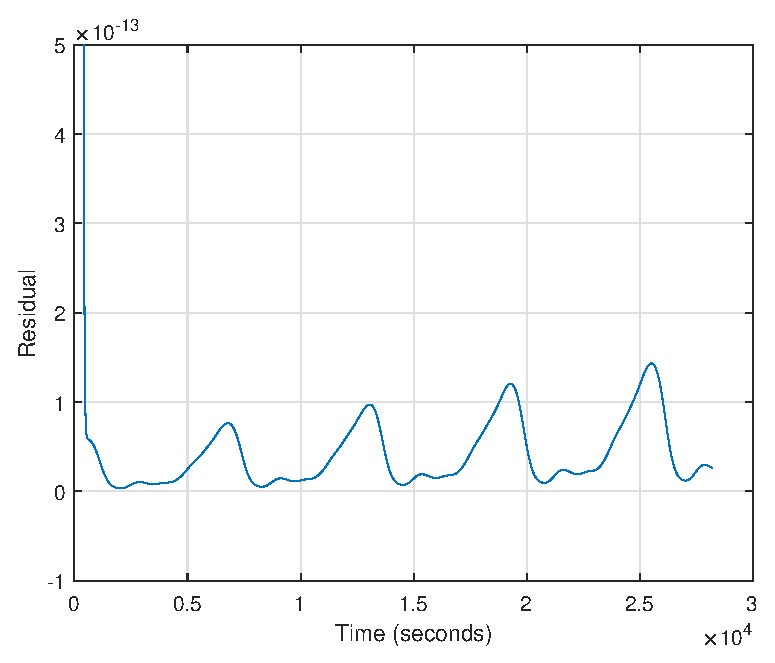
\includegraphics[width=0.7\linewidth]{figures/constdistonly_res}
%	\caption{only dist const}
%	\label{fig:residualdist}
%\end{figure}

%\begin{figure}[H]
%	\centering
%	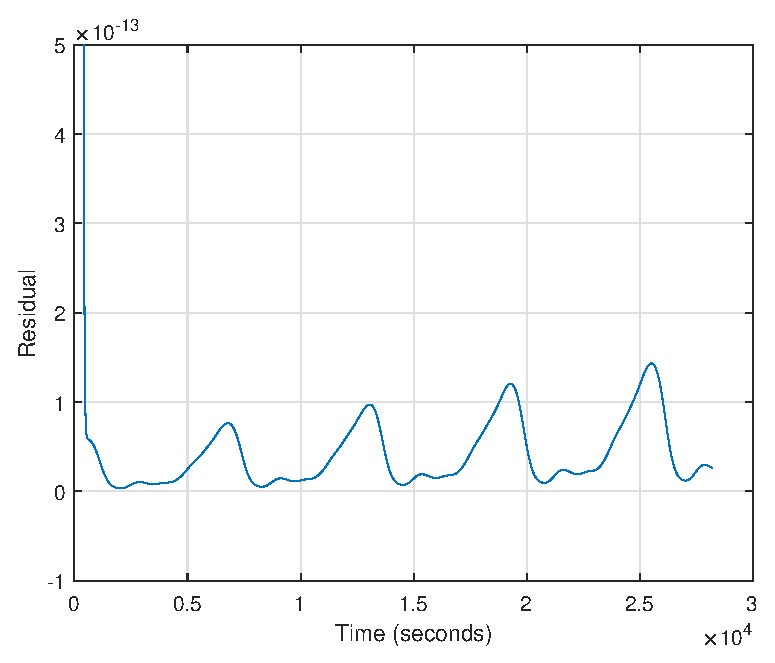
\includegraphics[width=0.7\linewidth]{figures/constdistonly_res}
%	\caption{only dist const}
%	\label{fig:residualdist}
%\end{figure}

%\begin{figure}[H]
%	\centering
%	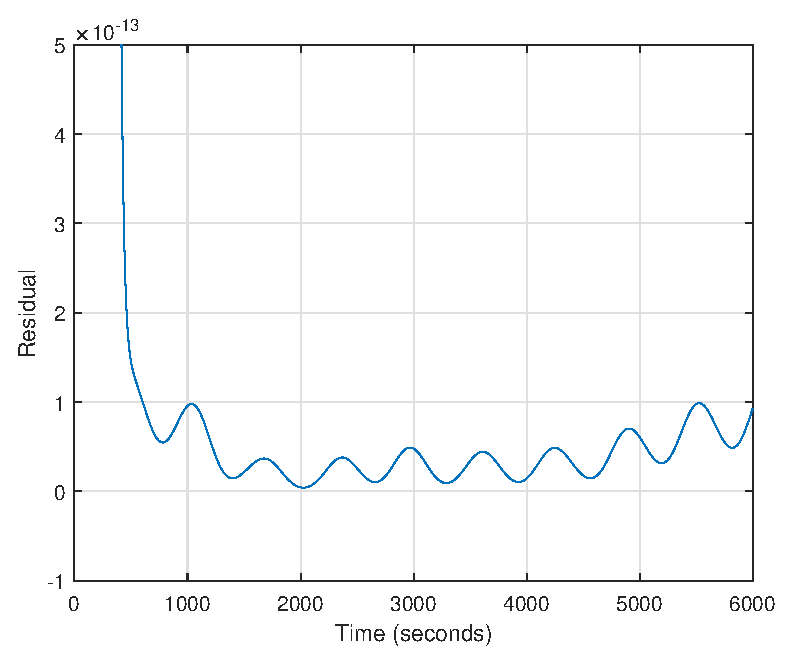
\includegraphics[width=0.7\linewidth]{figures/distonly_res}
%	\caption{only dist sine}
%	\label{fig:}
%\end{figure}

%\nomenclature[Sw]{$\omega_o$}{Orbit angular velocity}

%
%\tiny
%\begin{align}
%\begin{bmatrix}
%\vec{_{lv}^s\dot{\omega}} \\
%\vec{\dot{\omega}_{rw} } \\
%\vec{\dot{q}_{1:3}}
%\end{bmatrix} 
%\nonumber
%= \begin{bmatrix}
%0 & 0 & \omega_o\frac{I_1 - I_2 + I_3}{-I_1} & 0 & 0 & \omega_o\frac{I_w}{-I_1} & 8\omega_o^2\frac{I_3 - I_2}{I_1} & 0 & 0 \\
%0 & 0 &	0 & 0 & 0 &	0 & 0 &  6\omega_o^2\frac{I_3 - I_1}{I_2} & 0\\
%\omega_o\frac{I_1 - I_2 + I_3}{I_3}  & 0 & 0 &  \omega_o\frac{I_w}{I_3} & 0 &	0 & 0 & 0 & 2\omega_o^2\frac{I_1 - I_2}{I_3}\\
%0 & 0 &	0  & 0 & 0 & 0 & 0 & 0 & 0\\
%0 & 0 &	0  & 0 & 0 & 0 & 0 & 0 & 0 \\
%0 & 0 &	0 & 0 & 0 & 0 & 0 & 0 & 0\\
%0.5 & 0 &	0 & 0 & 0 & 0 & 0 & 0 & 0 \\
%0 & 0.5 &	0& 0 & 0 & 0 & 0 & 0 & 0 \\
%0 & 0 &	0.5 & 0 & 0 & 0 & 0 & 0 & 0\\
%\end{bmatrix}
%\begin{bmatrix}
%_{lv}^s\omega_1 \\
%_{lv}^s\omega_2 \\
%_{lv}^s\omega_3 \\
%\omega_{rw,1} \\
%\omega_{rw,2} \\
%\omega_{rw,3} \\
%q_1 \\
%q_2 \\
%q_3 
%\end{bmatrix}
%\\
%\nonumber
%+
%\begin{bmatrix}
%I_1^{-1} & 0 & 0 & 0 & \frac{b_3}{I_1} & -\frac{b_2}{I_1}	& I_1^{-1} & 0 & 0\\
%0 & I_2^{-1} & 0 & - \frac{b_3}{I_2} & 0 &  \frac{b_1}{I_2} & 0 & I_2^{-1} & 0\\ 
%0 & 0 & I_3^{-1} &  \frac{b_2}{I_3} &  -\frac{b_1}{I_3} & 0 & 0 & 0 & I_3^{-1} \\  
%I_w^{-1} & 0 & 0 & 0 & 0 & 0 & 0 & 0 & 0 \\
%0 & I_w^{-1} & 0 & 0 & 0 & 0 & 0 & 0 & 0 \\ 
%0 & 0 & I_w^{-1} & 0 & 0 & 0 & 0 & 0 & 0\\  
%0 & 0 & 0 & 0 & 0 & 0 & 0 & 0 & 0\\
%0 & 0 & 0 & 0 & 0 & 0 & 0 & 0 & 0\\
%0 & 0 & 0 & 0 & 0 & 0 & 0 & 0 & 0\\
%\end{bmatrix}
%\begin{bmatrix}
%N_{rw,1} \\
%N_{rw,2} \\
%N_{rw,3}\\
%\m_{mt,1} \\
%\m_{mt,2} \\
%\m_{mt,3} \\
%N^{est}_{dist,1} \\
%N^{est}_{dist,2} \\
%N^{est}_{dist,3}
%\end{bmatrix}
%+
%\begin{bmatrix}
%I_1^{-1} & 0 & 0 \\
%0 & I_2^{-1} & 0 \\
%0 & 0 & I_3^{-1}\\
%0 & 0 & 0 \\
%0 & 0 & 0 \\
%0 & 0 & 0 \\
%0 & 0 & 0 \\
%0 & 0 & 0 \\
%0 & 0 & 0 
%\end{bmatrix}
%\begin{bmatrix}
%N^{est \ error}_{dist,1} \\
%N^{est \ error}_{dist,2} \\
%N^{est \ error}_{dist,3}\\
%\end{bmatrix}
%\\
%+ 
%\begin{bmatrix}
%I_1^{-1} & 0 & 0 & 0 & \frac{b_3}{I_1} & -\frac{b_2}{I_1}\\
%0 & I_2^{-1} & 0 & - \frac{b_3}{I_2} & 0 &  \frac{b_1}{I_2} \\ 
%0 & 0 & I_3^{-1} &  \frac{b_2}{I_3} &  -\frac{b_1}{I_3} & 0 \\  
%I_w^{-1} & 0 & 0 & 0 & 0 & 0 \\
%0 & I_w^{-1} & 0 & 0 & 0 & 0 \\ 
%0 & 0 & I_w^{-1} & 0 & 0 & 0 \\  
%0 & 0 & 0 & 0 & 0 & 0 \\
%0 & 0 & 0 & 0 & 0 & 0 \\
%0 & 0 & 0 & 0 & 0 & 0 \\
%\end{bmatrix}
%\begin{bmatrix}
%N^{fault}_{rw,1} \\
%N^{fault}_{rw,2} \\
%N^{fault}_{rw,3}\\
%\m^{fault}_{mt,1} \\
%\m^{fault}_{mt,2} \\
%\m^{fault}_{mt,3} 
%\end{bmatrix}
%\label{eq:uioMatrices}
%\end{align}
%\normalsize